% =============================================================================
%  BÁO CÁO NGẮN (tiếng Việt) - Mô hình xác suất cho lexicon của rule engine
%  và ảnh hưởng của nó lên hệ thống fusion.
%
%  Đối tượng đọc: mentor / hội đồng. Mục tiêu: giải thích rõ RÀNG VÀ TRUNG THỰC
%  vì sao một cải thiện CÓ Ý NGHĨA ở rule engine lại KHÔNG truyền lên fusion.
%
%  BIÊN DỊCH (khuyến nghị - XeLaTeX, hỗ trợ tiếng Việt tốt nhất):
%      xelatex bao_cao_mo_hinh_xac_suat.tex
%      xelatex bao_cao_mo_hinh_xac_suat.tex      % chạy 2 lần để ổn định tham chiếu
%
%  (Có thể dùng pdflatex, nhưng khi đó bỏ khối polyglossia/fontspec và thay bằng
%   \usepackage[utf8]{inputenc} + \usepackage[T5]{fontenc}
%   + \usepackage[vietnamese]{babel} - xem README.md.)
%
%  Mọi con số trong báo cáo được sao CHÉP NGUYÊN VĂN từ các tệp JSON/MD đã sinh
%  bởi scripts 40-44. Không có số nào được tính lại bằng tay ở đây.
% =============================================================================
\documentclass[11pt,a4paper]{article}

% ---- Hỗ trợ tiếng Việt (XeLaTeX) ------------------------------------------- %
\usepackage{fontspec}
\usepackage{polyglossia}
\setmainlanguage{vietnamese}
\setotherlanguage{english}
% Nếu máy không có font Times New Roman, đổi thành \setmainfont{Latin Modern Roman}
\setmainfont{Times New Roman}
\setsansfont{Arial}
\setmonofont{Consolas}

% ---- Gói thông dụng -------------------------------------------------------- %
\usepackage{graphicx}
\usepackage{booktabs}
\usepackage{array}
\usepackage{multirow}
\usepackage{amsmath}
\usepackage{amssymb}
\usepackage{xcolor}
\usepackage{tikz}
\usetikzlibrary{arrows.meta,positioning,fit,backgrounds,calc}
\usepackage{caption}
\usepackage{float}
\usepackage{enumitem}
\usepackage{geometry}
\usepackage[hidelinks]{hyperref}

\geometry{margin=2.4cm}
\captionsetup{font=small,labelfont=bf}
\setlength{\parskip}{0.35em}
\setlength{\parindent}{0pt}

% ---- Màu & macro ----------------------------------------------------------- %
\definecolor{cok}{HTML}{2CA02C}     % xanh: có ý nghĩa
\definecolor{cfail}{HTML}{C44E52}   % đỏ: không ý nghĩa
\definecolor{cbase}{HTML}{4C72B0}   % xanh dương: mốc
\definecolor{cgray}{HTML}{7F7F7F}

\newcommand{\ok}[1]{\textcolor{cok}{\textbf{#1}}}
\newcommand{\bad}[1]{\textcolor{cfail}{\textbf{#1}}}
\newcommand{\code}[1]{\texttt{\small #1}}
% Cho phép giãn dòng nhẹ ở các đoạn chứa đường dẫn dài.
\sloppy
\newcommand{\sys}[1]{\textsc{#1}}

\title{\textbf{Mô hình xác suất Naive Bayes cho lexicon của rule engine\\
       và ảnh hưởng của nó lên hệ thống fusion}\\[0.4em]
       \large Báo cáo ngắn kỹ thuật (tiếng Việt)}
\author{SensitiveAI --- Capstone Project\\ \small Báo cáo nội bộ cho mentor}
\date{21 tháng 10, 2026}

\begin{document}
\maketitle

% =============================================================================
\begin{abstract}
\noindent
Báo cáo này trình bày một hướng cải thiện hệ thống phát hiện ngôn từ thù địch
tiếng Việt bằng một \emph{mô hình xác suất} (Naive Bayes trên bag-of-words) sinh
lexicon cho rule engine, thay cho việc gán nhãn thủ công hoặc bằng
tần suất.  Kết quả chính gồm hai phần, và phần thứ hai quan trọng hơn:
(i)~ở tầng \textbf{rule engine}, lexicon sinh bởi Naive Bayes nâng macro-F1 trên
validation từ $0.4555$ lên $0.4800$ ($\Delta=+0.0245$, CI 95\% $[+0.0012,+0.0476]$,
$p=0.038$) --- \ok{một cải thiện có ý nghĩa thống kê};
(ii)~nhưng ở tầng \textbf{fusion} (hệ thống cuối), cùng thay đổi đó chỉ đưa
macro-F1 test từ $0.6647$ lên $0.6677$ ($\Delta=+0.0030$, CI 95\%
$[-0.0035,+0.0094]$, $p=0.351$) --- \bad{không có ý nghĩa}.
Báo cáo phân tích vì sao: rule engine dù mạnh lên vẫn \emph{yếu hơn} nhánh AI,
và nút thắt thật nằm ở lớp \textsc{offensive}.  Chúng tôi trình bày kiến trúc
hệ thống, công thức Naive Bayes, ngưỡng multi-label, toàn bộ chuỗi bốn hướng đã
thử, cùng các hình minh hoạ.  Đây là một \emph{kết quả âm trung thực}, có giá
trị định hướng: muốn nâng điểm hệ thống cuối, cần cải thiện nhánh AI/head cho
lớp \textsc{offensive}, không phải tiếp tục mở rộng lexicon.
\end{abstract}

% =============================================================================
\section{Đặt vấn đề và câu hỏi nghiên cứu}
\label{sec:intro}

Hệ thống của chúng tôi phân loại bình luận tiếng Việt thành ba lớp
\textsc{hate} / \textsc{offensive} / \textsc{clean}.  Nhánh chính là một mô hình
học sâu (encoder \code{microsoft/mdeberta-v3-base} + head nhiều góc nhìn).
Song song, hệ thống có một \textbf{rule engine} dựa trên từ điển (lexicon): nó
đối chiếu văn bản với danh sách term độc hại rồi cho điểm từng lớp.  Hai nhánh
được hợp nhất bằng một khối \textbf{fusion} (Hình~\ref{fig:arch}).

Lexicon hiện tại gồm \textbf{668 term} gán nhãn thủ công.  Hạn chế hiển nhiên:
nó nhỏ, tốn công, và mỗi term chỉ mang \emph{một} nhãn.  Mentor gợi ý:

\begin{quote}
\emph{``Có thể nằm ở nhiều label + dùng mô hình xác suất để tính xem từ đó
thuộc nhãn nào?''}
\end{quote}

Từ đó câu hỏi nghiên cứu của báo cáo:

\begin{description}[leftmargin=1.4em,style=nextline]
  \item[Câu hỏi 1.] Một \emph{mô hình xác suất} (Naive Bayes) có sinh được
  lexicon tốt hơn cách gán nhãn hiện tại, đo trên rule engine không?
  \item[Câu hỏi 2.] Nếu rule engine tốt lên, \emph{điểm hệ thống cuối} (fusion)
  có tốt lên tương xứng không?
  \item[Câu hỏi 3.] Multi-label có phải là nguồn cải thiện không, và nút thắt
  thật sự của cả hệ thống nằm ở đâu?
\end{description}

Trả lời ngắn gọn: (1)~có, và có ý nghĩa thống kê; (2)~\bad{không} --- cải thiện
không truyền lên fusion; (3)~multi-label \emph{không} phải nguồn cải thiện, nút
thắt thật là lớp \textsc{offensive} và nhánh AI.

% =============================================================================
\section{Kiến trúc hệ thống}
\label{sec:arch}

Hình~\ref{fig:arch} vẽ kiến trúc thật của hệ thống.  Có hai nhánh song song,
được hợp nhất ở cuối.

\begin{figure}[H]
  \centering
  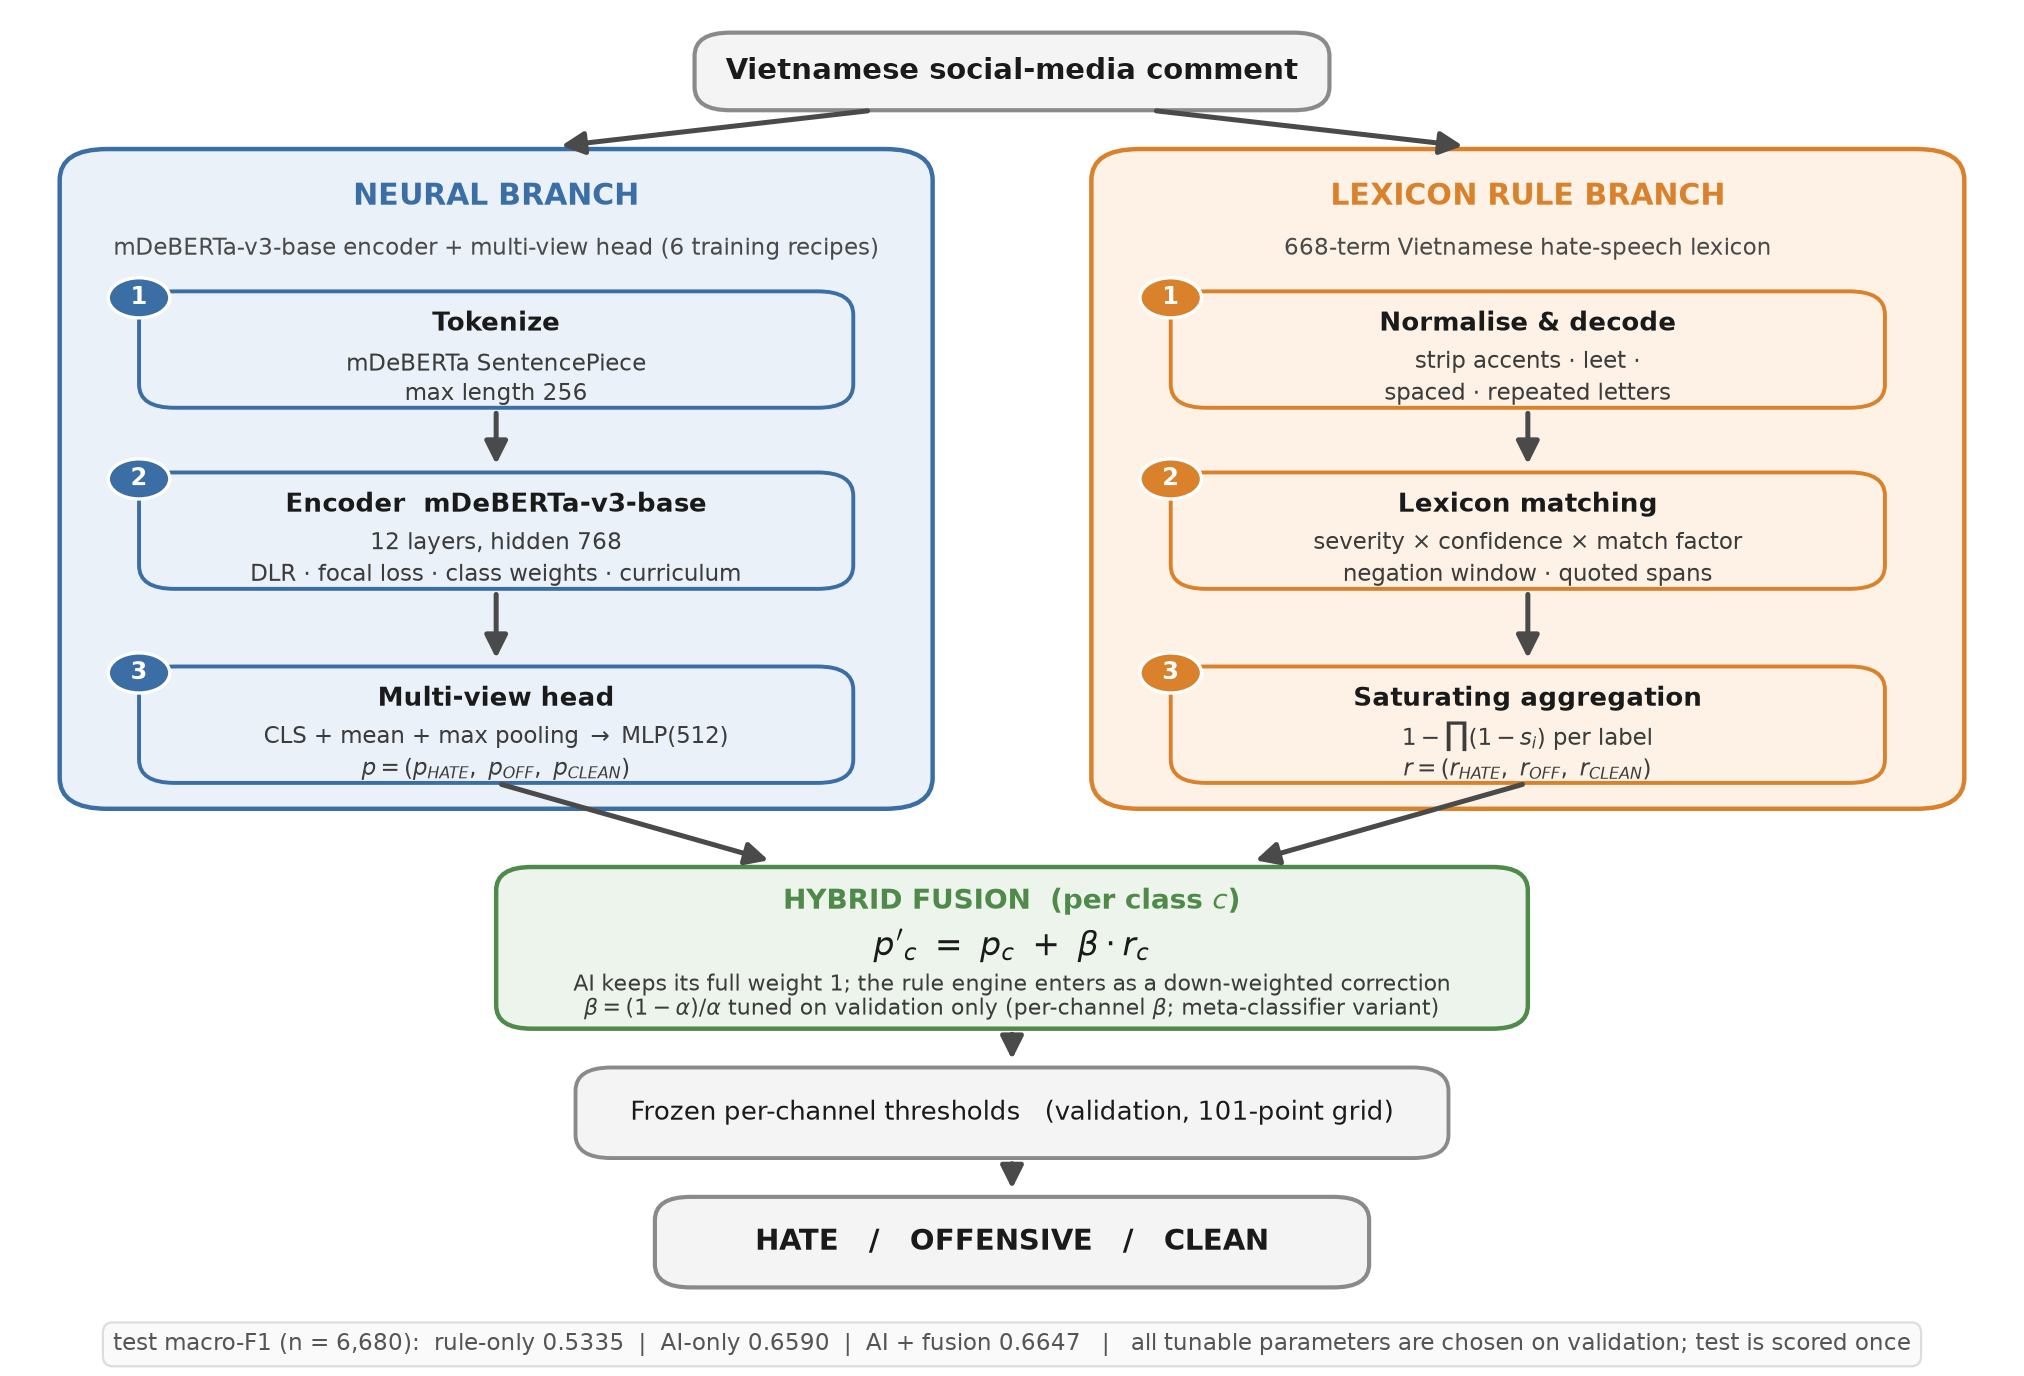
\includegraphics[width=0.98\textwidth]{figures/system_architecture.png}
  \caption{Kiến trúc toàn hệ thống.  \textbf{Nhánh AI} (trên): encoder
  \code{mdeberta-v3-base} + head nhiều góc nhìn (cls + mean + max) cho ra phân
  phối xác suất $p$.  \textbf{Nhánh rule} (dưới): chuẩn hoá $\rightarrow$ lexicon
  $\rightarrow$ điểm rule $r$ cho từng lớp, có xử lý obfuscation (mất dấu, leet,
  lặp ký tự).  \textbf{Fusion} hợp nhất theo công thức
  $p' = p + \beta\,r$ (nhánh AI giữ trọng số 1, nhánh rule bị hạ trọng số $\beta$)
  rồi áp ngưỡng quyết định \emph{theo từng kênh} (per-channel thresholds) đã
  chốt trên validation.  Hình do \code{scripts/30\_plot\_system\_architecture.py}
  sinh trực tiếp từ định nghĩa hệ thống (không vẽ tay).}
  \label{fig:arch}
\end{figure}

\subsection{Nhánh AI}
Encoder \code{mdeberta-v3-base} (278{,}2M tham số) sinh biểu diễn chuỗi, sau đó
head \emph{nhiều góc nhìn} gộp ba vector: token đầu \textsc{cls}, trung bình có
mặt nạ (masked mean) và max có mặt nạ (masked max).  Ba vector được nối thành
một vector 2304 chiều, đi qua khối
$\mathrm{Linear}(2304{\to}512)\to\mathrm{GELU}\to\mathrm{Dropout}$, rồi
$\mathrm{Linear}(512{\to}3)$ cho ra xác suất 3 lớp.  Kết quả là phân phối
$p=(p_{\textsc{hate}},p_{\textsc{offensive}},p_{\textsc{clean}})$.

\subsection{Nhánh rule engine}
Nhánh này gồm ba bước:
\begin{enumerate}[leftmargin=1.6em]
  \item \textbf{Chuẩn hoá văn bản}: Unicode NFC, viết thường, bỏ ký tự vô hình,
  gộp khoảng trắng, giới hạn ký tự lặp (\code{nguuuu}$\to$\code{nguu}).
  \item \textbf{Đối chiếu lexicon} qua nhiều ``góc nhìn chống obfuscation'':
  khớp chính xác, bỏ dấu, leet (\code{c0n ch0}), gộp ký tự lặp, chèn dấu phân
  cách, và fuzzy (khoảng cách $\le 1$).  Mỗi kiểu khớp có một hệ số tin cậy
  riêng (\code{match\_factors}).
  \item \textbf{Cho điểm}: mỗi kết quả khớp có điểm
  \[
    s = \underbrace{\text{severity}}_{\text{mức độ nhãn}}
        \times \underbrace{c}_{\text{confidence của term}}
        \times \underbrace{f}_{\text{hệ số kiểu khớp}}
        \times \underbrace{k}_{\text{hệ số ngữ cảnh (phủ định/trích dẫn)}},
  \]
  rồi gộp về điểm từng lớp bằng tổng bão hoà
  \[
    r_{\text{label}} = 1 - \prod_{i=1}^{n}\bigl(1 - s_i\bigr),
    \qquad n \le \text{aggregation\_cap} = 10 .
  \]
  Công thức này \emph{bão hoà}: càng nhiều term khớp thì điểm tiến gần 1 nhưng
  không vượt quá 1.  Cuối cùng rule engine cho ra $r=(r_{\textsc{hate}},
  r_{\textsc{offensive}},r_{\textsc{clean}})$.
\end{enumerate}

\subsection{Fusion}
Fusion trộn hai nhánh.  Bản đang dùng là \emph{per-channel}:
\[
  p'_{c} = \alpha_c\, p_{c} + (1-\alpha_c)\, r_{c},
\]
trong đó $\alpha_c$ là trọng số tin nhánh AI \emph{riêng cho từng lớp} $c$, và
$r$ đã được ``làm sạch'' theo $r_{\text{clean}} = 1 - \max(r_{\text{hate}},
r_{\text{offensive}})$ để tránh mâu thuẫn giữa các lớp.  Sau đó áp ngưỡng quyết
định per-channel đã chốt trên validation.  Trong báo cáo này, bước ``quyết
định'' (ngưỡng) đã được tối ưu trên \emph{validation} và \emph{đóng băng} trước
khi chấm \emph{test}, đúng theo giao thức ở mục~\ref{sec:protocol}.

% =============================================================================
\section{Mô hình xác suất Naive Bayes cho lexicon}
\label{sec:nb}

\subsection{Ý tưởng}
Thay vì gán nhãn lexicon bằng tay hoặc bằng tần suất thô, ta \emph{học} phân
phối xác suất ``một term thuộc lớp nào'' từ chính corpus huấn luyện
(ViHSD + ViCM + Bontori, 135{,}238 dòng).  Corpus được token hoá đơn giản thành
\emph{syllable} và \emph{bigram/trigram}; mỗi term ứng viên (term cũ + term
sinh bởi bước tokenize) được chấm điểm Naive Bayes.

\subsection{Công thức}
Với lớp $c\in\{\textsc{hate},\textsc{offensive},\textsc{clean}\}$, gọi
$\mathrm{df}_c(\text{term})$ là số dòng thuộc lớp $c$ chứa term, $N_c$ là số dòng
lớp $c$, $V$ là kích thước từ vựng, $\alpha$ là hệ số làm trơn Laplace:

\[
  P(\text{term}\mid c) = \frac{\mathrm{df}_c(\text{term}) + \alpha}{N_c + \alpha V},
  \qquad
  P(\text{term}) = \frac{\mathrm{df}(\text{term}) + \alpha}{N_{\text{all}} + \alpha V}.
\]

\textbf{Điểm quan trọng --- dùng log-odds, không dùng posterior thô.}  Vì corpus
rất lệch (khoảng 83\% là \textsc{clean}), nếu dùng posterior thô thì tiên nghiệm
$P(c)$ sẽ kéo mọi term về \textsc{clean}.  Do đó ta dùng \emph{lift}:

\[
  \ell_c(\text{term}) = \log P(\text{term}\mid c) - \log P(\text{term}).
\]

Log-odds đã ``chia'' cho $P(\text{term})$ chung, nên nó đo mức term xuất hiện ở
lớp $c$ \emph{nhiều hơn hẳn} các lớp khác bao nhiêu --- đúng thứ ta cần cho
lexicon.  Sau đó chuẩn hoá về phân phối qua softmax:
\[
  P(c\mid\text{term}) = \frac{\exp\bigl(\ell_c - \max_{c'}\ell_{c'}\bigr)}
                              {\sum_{c'}\exp\bigl(\ell_{c'} - \max_{c'}\ell_{c'}\bigr)} .
\]
(Trừ max để ổn định số học, không đổi kết quả.)

\subsection{Multi-label bằng ngưỡng}
Cách cũ dùng $\arg\max$: mỗi term chỉ giữ \emph{một} nhãn.  Cách mới
\emph{multi-label}: giữ \textbf{mọi} lớp $c$ có $P(c\mid\text{term}) \ge
\theta$ (ngưỡng $\theta$, ta gọi là \code{min\_prob}).  Đây chính là chỗ tận
dụng hạ tầng có sẵn: matcher trong \code{src/rule\_engine/matcher.py} đã lặp
\code{for label in entry.labels}, nên một term hoàn toàn có thể mang hai nhãn
\textsc{hate;offensive} và được cộng điểm cho cả hai lớp.

Ví dụ term ``hai nhãn'' thật trong dữ liệu: các tiếng chửi đa nghĩa như
\code{dm}, \code{vl} xuất hiện nhiều ở \emph{cả} hai lớp --- đúng thứ mà
$\arg\max$ trước đây làm mất.

\subsection{Lexicon thu được}
Với $\alpha=1.0$ và $\theta=0.25$ (cấu hình khảo sát ban đầu), ta thu được
\textbf{1{,}308 entry}, trong đó \textbf{585 term mang hai nhãn}.  Phân bố top-1
trước khi multi-label hoá: \textsc{hate} 804, \textsc{offensive} 295,
\textsc{clean} 329.  Một vài term xác suất cao (Bảng~\ref{tab:terms}).

\begin{table}[H]
  \centering
  \small
  \caption{Ví dụ term có xác suất cao nhất theo mô hình Naive Bayes
  (script 40, corpus ViHSD+ViCM+Bontori).  ``Nhãn giữ'' là các lớp có
  $P\ge\theta$ được đưa vào lexicon.}
  \label{tab:terms}
  \begin{tabular}{llccc}
    \toprule
    term & nhãn giữ & $P(\textsc{hate})$ & $P(\textsc{off})$ & $P(\textsc{clean})$ \\
    \midrule
    \code{thằng mặt}      & \textsc{hate}              & 0.907 & 0.062 & 0.030 \\
    \code{thằng chó}      & \textsc{hate}              & 0.902 & 0.082 & 0.016 \\
    \code{con mẹ mày}     & \textsc{hate}              & 0.898 & 0.069 & 0.033 \\
    \code{máy tui}        & \textsc{offensive}         & 0.040 & 0.882 & 0.078 \\
    \code{bủm chúa}       & \textsc{offensive}         & 0.063 & 0.876 & 0.061 \\
    \code{ăn cắp content} & \textsc{offensive}         & 0.063 & 0.876 & 0.061 \\
    \bottomrule
  \end{tabular}
\end{table}

% =============================================================================
\section{Thiết lập thực nghiệm và giao thức chống rò rỉ}
\label{sec:protocol}

Toàn bộ thí nghiệm tuân thủ quy tắc: \textbf{chỉ tune trên validation; test chỉ
chấm một lần và không ghi đè số cũ}.

\begin{itemize}[leftmargin=1.6em]
  \item \textbf{Dữ liệu}: 2{,}672 dòng validation, 6{,}680 dòng test.
  \item \textbf{Tune}: hệ số làm trơn $\alpha$ và ngưỡng multi-label $\theta$
  được quét trên \emph{validation} (script 42).  Ngưỡng quyết định của rule
  engine cũng tái tối ưu trên validation.
  \item \textbf{Đóng băng}: sau khi chọn cấu hình tốt nhất trên validation,
  ngưỡng được \emph{đóng băng} rồi mới chấm test (script 17 chế độ test).
  \item \textbf{Không ghi đè}: mọi artifact mới ghi vào thư mục riêng
  (\code{rule\_engine\_nb/}, \code{fusion\_nb/}); số liệu SOTA cũ giữ nguyên.
  \item \textbf{Kiểm định}: paired bootstrap (macro-F1) + McNemar, 10{,}000
  bootstrap, dùng \code{src/evaluation/analysis.py}.
\end{itemize}

Hình~\ref{fig:evol} (Hướng~4) và Bảng~\ref{tab:directions} cho thấy lexicon NB
là hướng duy nhất vượt kiểm định.  Hình~\ref{fig:delta} là forest plot của
toàn bộ chuỗi.

% =============================================================================
\section{Kết quả}
\label{sec:results}

\subsection{Tầng 1 --- Rule engine: NB tốt lên CÓ Ý NGHĨA}
\label{sec:res-rule}

Bảng~\ref{tab:rule} so sánh lexicon hiện tại với lexicon NB, đo trên rule engine
\emph{đứng riêng} ở validation.

\begin{table}[H]
  \centering
  \small
  \caption{Lexicon sinh bởi Naive Bayes vs lexicon hiện tại, trên rule engine
  đứng riêng (validation, $n=2672$).  ``Argmax'' là biến thể mỗi term chỉ một
  nhãn; cột chính ``Macro-F1 (thr)'' tái tối ưu ngưỡng trên validation.}
  \label{tab:rule}
  \begin{tabular}{lccccccc}
    \toprule
    Lexicon & Entry & Macro-F1 (thr) & Macro-F1 (argmax) & Acc & F1 \textsc{hate} & F1 \textsc{off} & F1 \textsc{clean} \\
    \midrule
    current (668)          & 668  & \textbf{0.4555} & 0.3438 & 0.702 & 0.368 & 0.169 & 0.830 \\
    nb only (1308)         & 1308 & \ok{0.4782}     & 0.3881 & 0.755 & 0.404 & 0.168 & 0.863 \\
    current + nb           & 1310 & 0.4596          & 0.3432 & 0.754 & 0.362 & 0.153 & 0.864 \\
    nb multilabel only     & 585  & 0.4498          & 0.4191 & 0.808 & 0.327 & 0.122 & 0.900 \\
    \bottomrule
  \end{tabular}
\end{table}

\textbf{Diễn giải:}
\begin{itemize}[leftmargin=1.6em]
  \item \textbf{nb only} (dùng \emph{toàn bộ} lexicon NB): $0.4782$ vs $0.4555$
  $\Rightarrow \Delta=+0.0227$, CI 95\% $[+0.0013,+0.0438]$, $p=0.037$
  (McNemar $234/92$, $p<0.001$) \ok{$\Rightarrow$ CÓ ý nghĩa}.
  \item \textbf{current + nb} (giữ cả lexicon cũ): \bad{$\Delta=+0.0042$,
  CI chứa 0, $p=0.702$} $\Rightarrow$ không ý nghĩa.  Nghĩa là lexicon NB
  \emph{thay thế} tốt hơn là \emph{bổ sung} vào lexicon cũ.
  \item \textbf{nb multilabel only} (chỉ giữ 585 term mang \emph{hai} nhãn):
  \bad{$\Delta=-0.0057$, CI chứa 0} $\Rightarrow$ giữ riêng term hai nhãn là
  \emph{không} đủ --- chốt lại multi-label \emph{không} phải nguồn cải thiện.
\end{itemize}

\subsection{Tầng 1 (tuned) --- điểm tốt nhất trên validation}
\label{sec:res-tuned}

Script 42 quét $\alpha \times \theta$ trên validation (Hình~\ref{fig:delta},
cột ``Hướng~4 tuned'').  Kết quả tốt nhất: $\alpha=0.3$, $\theta=0.35$
$\Rightarrow$ \textbf{1{,}155 entry, 208 term hai nhãn}, macro-F1 \ok{0.4800}
($\Delta=+0.0245$, CI 95\% $[+0.0012,+0.0476]$, $p=0.038$; McNemar $235/78$).

Một quan sát quan trọng: \textbf{9/12} cấu hình đều cải thiện rule engine, và
macro-F1 gần như phẳng theo cặp $(\alpha,\theta)$ --- trừ cấu hình $\theta=0.50$
\bad{(0 term hai nhãn) sụp $-0.049$}.  Điều này cho thấy:
\emph{mô hình xác suất} mới là thứ giúp, còn multi-label chỉ là \emph{hiệu ứng
phụ nhỏ}; và cần $\theta$ đủ thấp để giữ được các term hai nhãn.

\subsection{Tầng 2 --- Fusion: cải thiện KHÔNG truyền lên}
\label{sec:res-fusion}

Ta cắm lexicon NB (đã tune, 1155 entry) vào đúng nhánh rule của hệ thống, giữ
nguyên nhánh AI (dùng lại cache dự đoán, \emph{không} train lại), rồi chấm
fusion trên test.  Bảng~\ref{tab:fusion}.

\begin{table}[H]
  \centering
  \small
  \caption{Đo trên \textbf{test} ($n=6680$), cả hai hệ thống dùng chung cache dự
  đoán AI, nên chênh lệch \emph{chỉ} đến từ lexicon của rule engine.}
  \label{tab:fusion}
  \begin{tabular}{lcccc}
    \toprule
    Hệ thống & Macro-F1 & F1 \textsc{hate} & F1 \textsc{off} & F1 \textsc{clean} \\
    \midrule
    fusion SOTA (lexicon 668)  & 0.6647 & 0.5920 & 0.4612 & 0.9408 \\
    fusion + NB (lexicon 1155) & \textbf{0.6677} & 0.6084 & 0.4535 & 0.9412 \\
    \midrule
    $\Delta$ & \bad{+0.0030} & +0.0164 & $-0.0077$ & +0.0004 \\
    \bottomrule
  \end{tabular}
\end{table}

Kiểm định: $\Delta=+0.0030$, CI 95\% $[-0.0035,+0.0094]$, $p=0.351$;
McNemar $29$ đúng $/25$ sai $(p=0.684)$ $\Rightarrow$ \bad{KHÔNG có ý nghĩa}.

\begin{figure}[H]
  \centering
  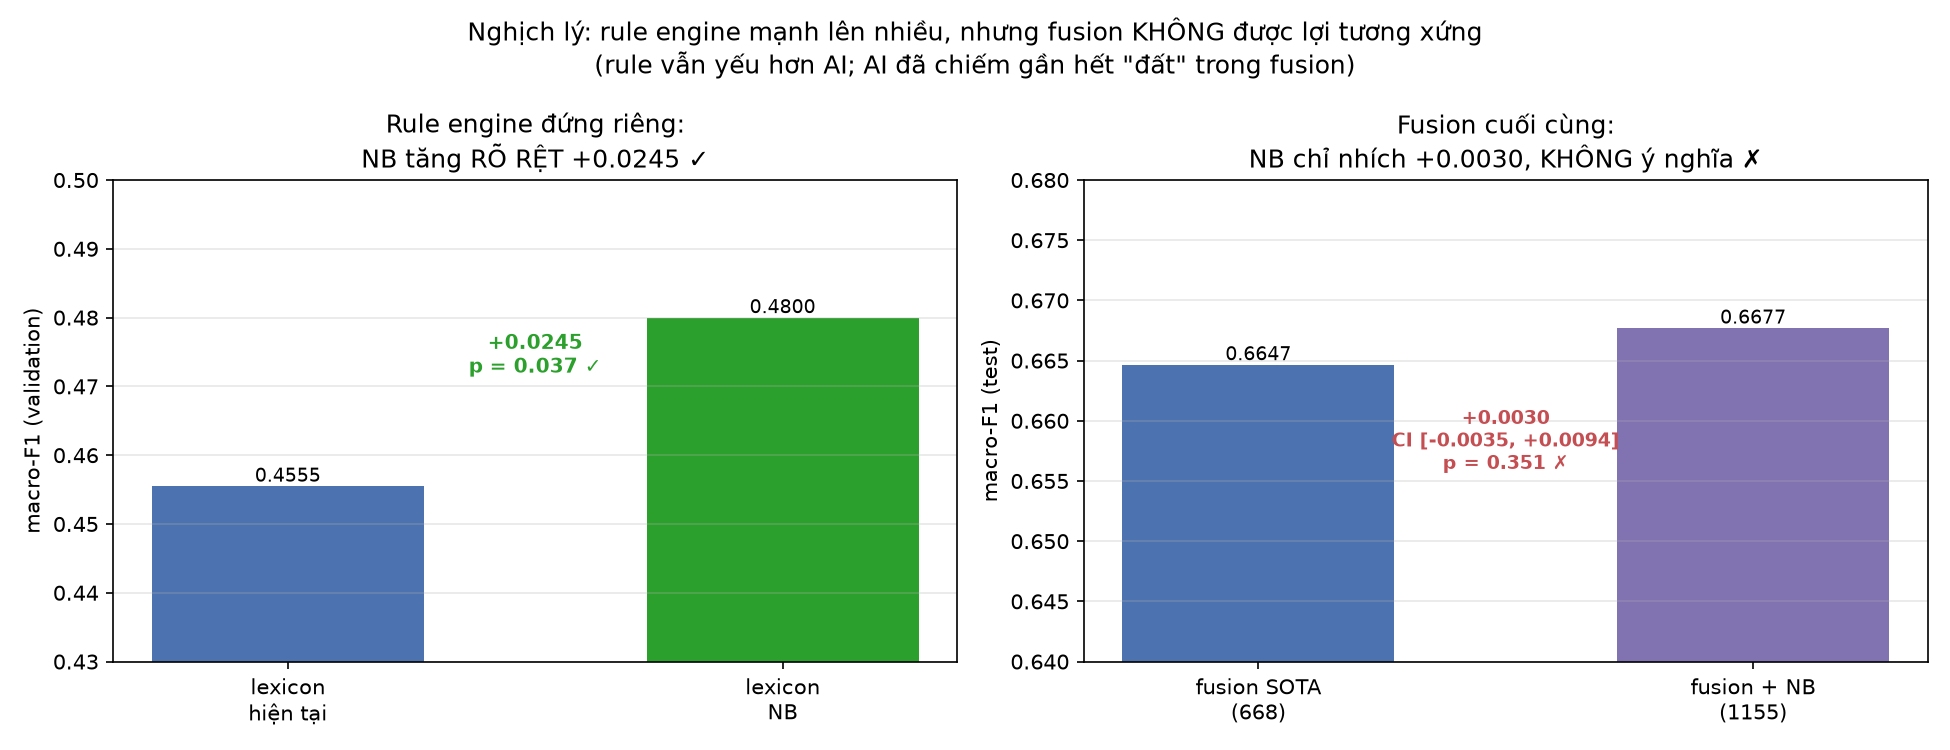
\includegraphics[width=0.98\textwidth]{figures/directions_rule_vs_fusion.png}
  \caption{\textbf{Nghịch lý cốt lõi.}  \emph{Trái}: trên rule engine đứng riêng,
  lexicon NB tăng \ok{+0.0245} ($p=0.037$, có ý nghĩa).  \emph{Phải}: trên fusion
  cuối cùng (test), cùng thay đổi chỉ nhích \bad{+0.0030} (không ý nghĩa).}
  \label{fig:rulevsfusion}
\end{figure}

% =============================================================================
\section{Phân tích: vì sao cải thiện ``bốc hơi'' ở fusion?}
\label{sec:why}

Đây là phần quan trọng nhất.  Rule engine mạnh lên $+0.047$ trên test
($0.5335\to0.5805$) nhưng fusion chỉ nhích $+0.0030$.  Có ba lý do, đều đo được:

\paragraph{(1) Rule engine vẫn yếu hơn nhánh AI.}
Trên test, rule engine NB đạt macro-F1 $0.5805$ còn nhánh AI đạt $0.6590$ (và
biến thể AI tốt nhất $0.6638$).  Rule dù mạnh lên vẫn là ``thành phần yếu''.  Khi
trộn một thành phần yếu (dù tốt hơn trước) vào một thành phần mạnh, cải thiện
biên thu được rất nhỏ.

Bằng chứng định lượng: fusion \emph{đã nhận ra} rule mạnh lên và \emph{chuyển
trọng số} sang rule --- trọng số tổng $\alpha$ đổi từ $0.9$ (SOTA) xuống $0.7$
(NB), và ở kênh \textsc{hate} trọng số AI tụt xuống $\alpha_{\textsc{hate}}=0.1$
(gần như tin rule hoàn toàn).  Nhờ vậy F1 \textsc{hate} trên test tăng
$0.5920\to0.6084$.  Nhưng fusion \emph{không thể} đẩy macro-F1 lên thêm.

\paragraph{(2) Rule engine vẫn rất yếu ở lớp \textsc{offensive}.}
F1 \textsc{offensive} của rule NB trên test chỉ $0.3142$.  Khi fusion chuyển bớt
trọng số sang rule, F1 \textsc{offensive} của hệ thống \emph{giảm}
($0.4612\to0.4535$).  Đây là cái giá của việc tin rule hơn.

\paragraph{(3) Nhánh AI đã chiếm gần hết ``đất''.}
Khoảng trống giữa AI-only ($0.6590$) và fusion ($0.6647$) chỉ $0.006$.  Rule
mạnh lên chỉ lấp được khoảng $1/2$ khoảng trống đó, và phần lấp vào lại bị lớp
\textsc{offensive} ăn mất.

\paragraph{Nút thắt thật.}  Hình~\ref{fig:perclass} cho thấy F1 lớp
\textsc{offensive} \emph{không} được cải thiện bởi \emph{bất kỳ} hướng lexicon
nào ($0.169\to0.175$).  Đây là nút thắt thật của cả hệ thống --- và nó nằm ở
nhánh AI/head, không ở rule engine.

\begin{figure}[H]
  \centering
  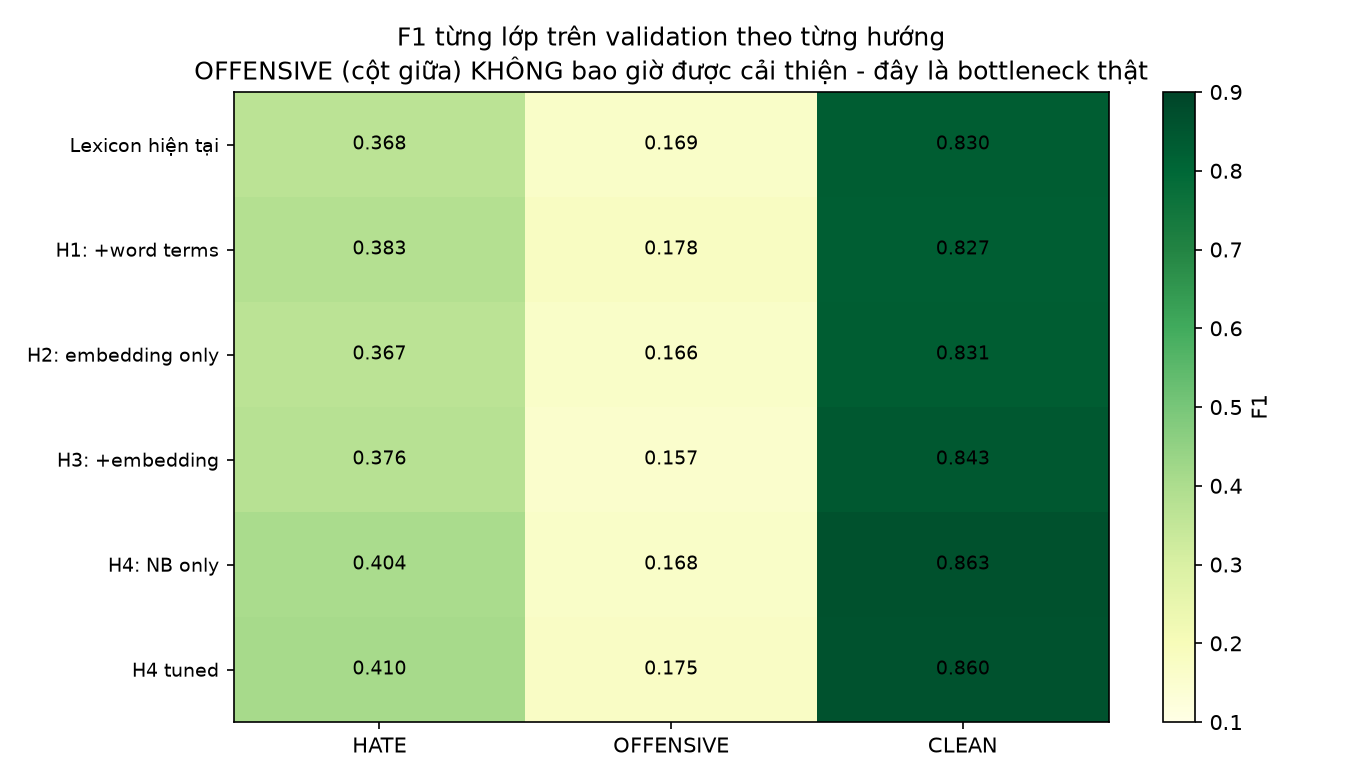
\includegraphics[width=0.92\textwidth]{figures/directions_per_class.png}
  \caption{Heatmap F1 từng lớp trên validation theo từng hướng lexicon.  Cột giữa
  (\textsc{offensive}) \emph{không bao giờ} đổi màu --- mọi hướng đều bó tay ở
  lớp này.  Đây là bằng chứng trực tiếp cho thấy nút thắt nằm ở
  \textsc{offensive}.}
  \label{fig:perclass}
\end{figure}

% =============================================================================
\section{Toàn bộ chuỗi bốn hướng đã thử}
\label{sec:chain}

Trước khi đi tới Naive Bayes, chúng tôi đã thử ba hướng khác (đều theo gợi ý
mở rộng lexicon).  Bảng~\ref{tab:directions} và Hình~\ref{fig:delta} tổng hợp
tất cả, đo trên rule engine đứng riêng ở validation.

\begin{table}[H]
  \centering
  \small
  \caption{Bốn hướng cải thiện lexicon, đo trên rule engine đứng riêng
  (validation, $n=2672$).  10{,}000 paired bootstrap.  Chỉ Hướng~4 vượt kiểm
  định.  (Dòng cuối là số đo trên fusion ở test.)}
  \label{tab:directions}
  \begin{tabular}{lcccc}
    \toprule
    Hướng & Macro-F1 & $\Delta$ & CI 95\% & Kết luận \\
    \midrule
    Lexicon hiện tại (mốc)              & 0.4555 & --- & --- & --- \\
    H1: tokenize VI + word terms        & 0.4628 & +0.0074 & $[-0.0045,+0.0192]$ & \bad{không} \\
    H2: fastText embedding only         & 0.4545 & $-0.0010$ & $[-0.0245,+0.0232]$ & \bad{không} \\
    H3: fastText + embedding            & 0.4585 & +0.0030 & $[-0.0196,+0.0263]$ & \bad{không} \\
    H4: NB xác suất + multi-label       & 0.4782 & +0.0227 & $[+0.0013,+0.0438]$ & \ok{có} \\
    H4 tuned ($\alpha=0.3,\theta=0.35$) & \textbf{0.4800} & +0.0245 & $[+0.0012,+0.0476]$ & \ok{có} \\
    \midrule
    \emph{Fusion SOTA (test)}           & 0.6647 & --- & --- & --- \\
    \emph{Fusion + NB (test)}           & 0.6677 & +0.0030 & $[-0.0035,+0.0094]$ & \bad{không} \\
    \bottomrule
  \end{tabular}
\end{table}

\begin{figure}[H]
  \centering
  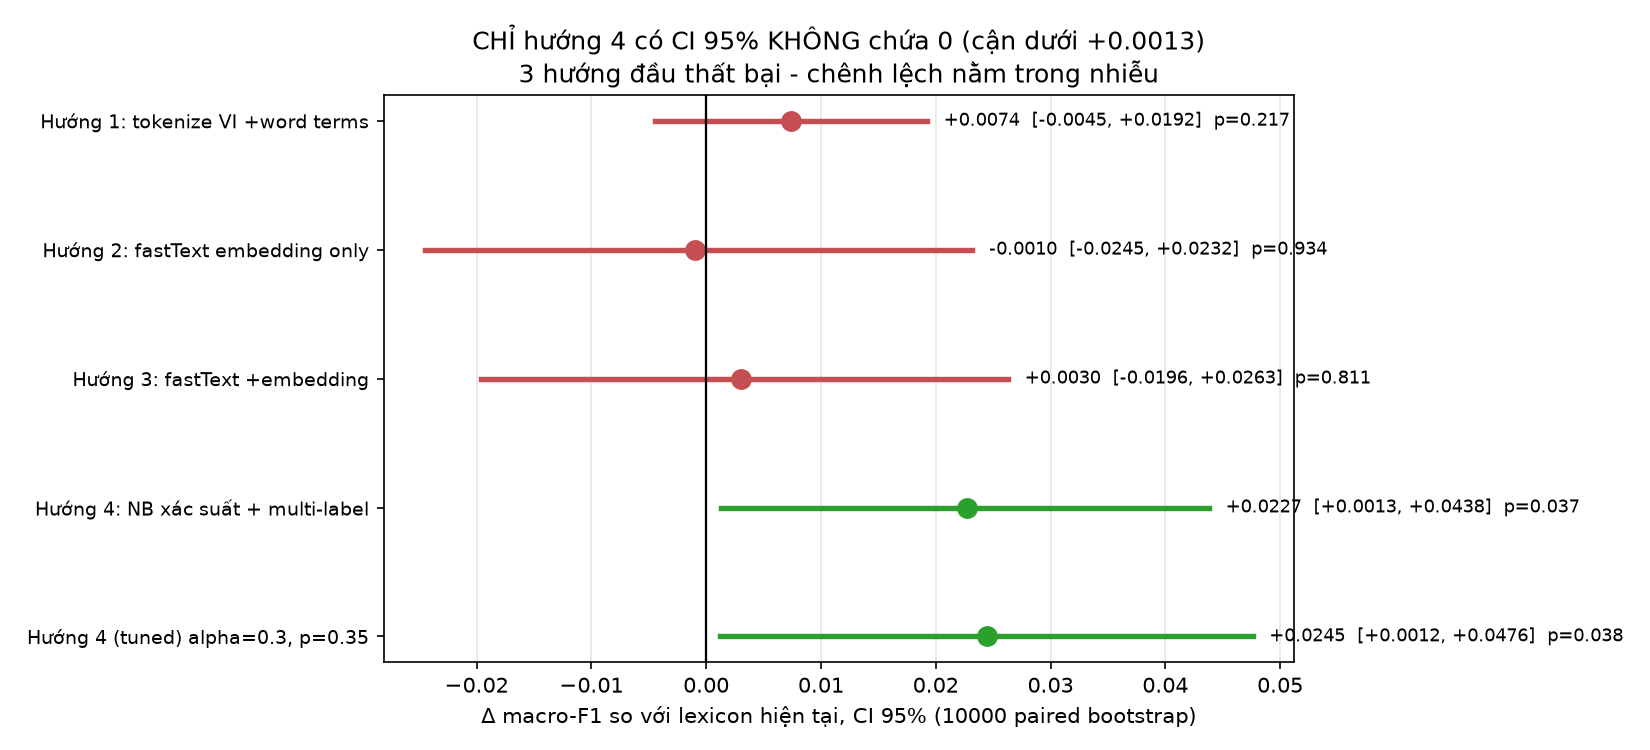
\includegraphics[width=0.98\textwidth]{figures/directions_delta_ci.png}
  \caption{Forest plot: $\Delta$ macro-F1 và CI 95\% của \emph{mọi} hướng so với
  lexicon hiện tại.  \textbf{Chỉ Hướng~4 có CI 95\% không chứa 0} (cận dưới
  $+0.0013$); ba hướng còn lại CI đều chứa 0, tức chênh lệch nằm trong nhiễu.}
  \label{fig:delta}
\end{figure}

\begin{figure}[H]
  \centering
  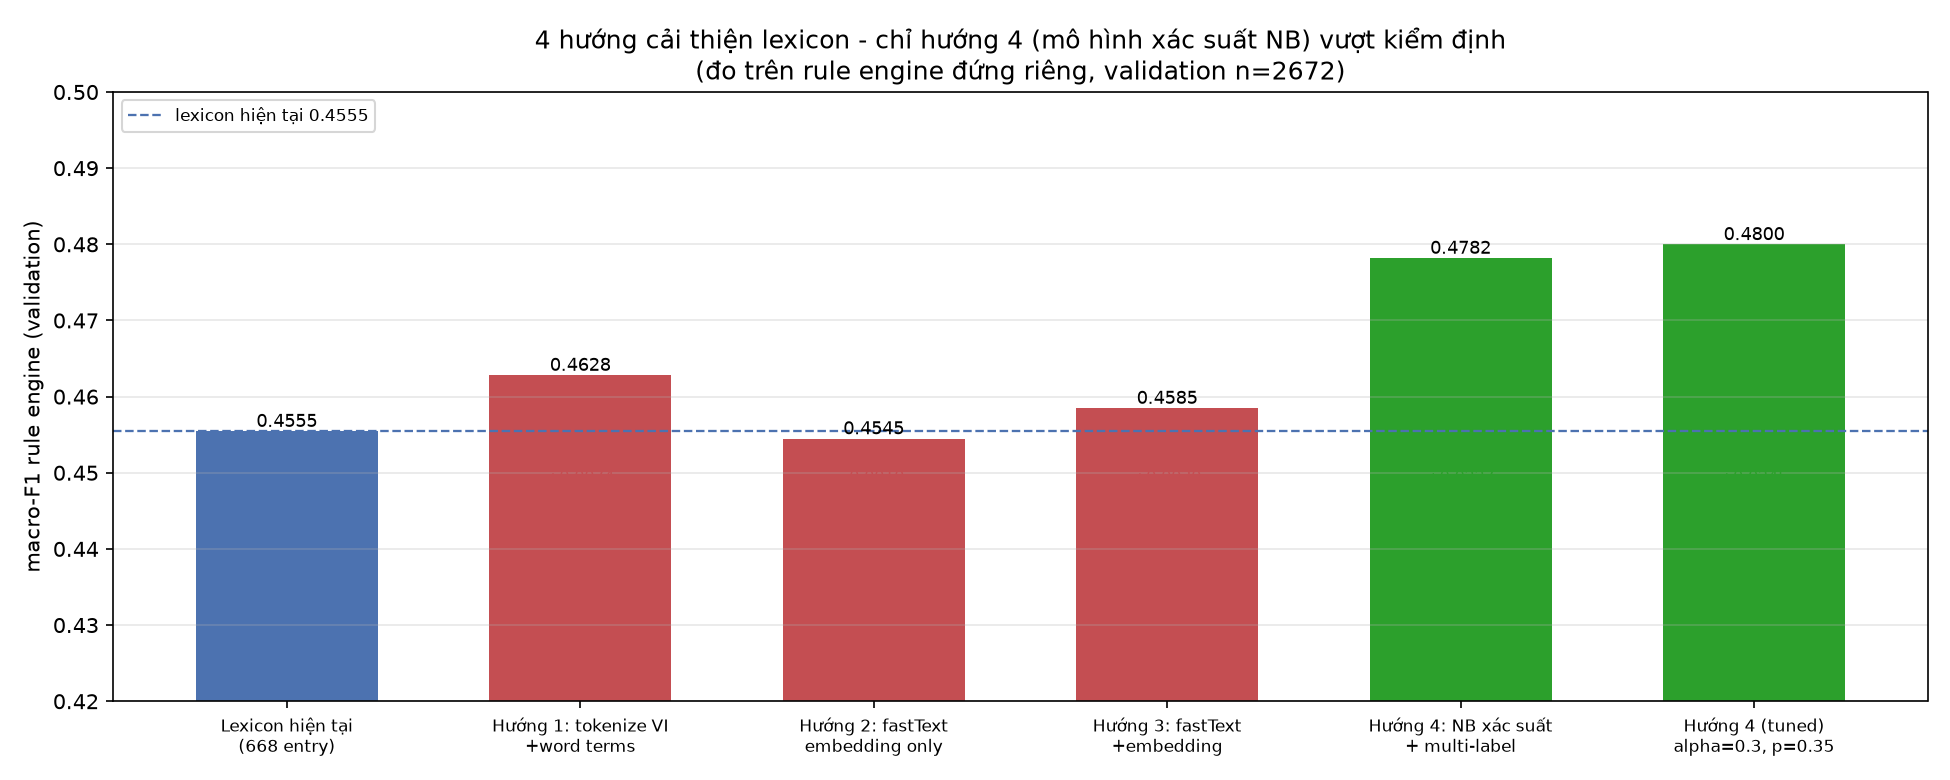
\includegraphics[width=0.98\textwidth]{figures/directions_evolution.png}
  \caption{macro-F1 của rule engine qua từng hướng (validation).  Cột xanh lá =
  hướng vượt kiểm định (Hướng~4), cột đỏ = hướng thất bại.  Đường đứt là mốc
  lexicon hiện tại $0.4555$.}
  \label{fig:evol}
\end{figure}

\textbf{Vì sao ba hướng đầu thất bại?}  Cả ba đều mắc một trong hai lỗi thiết kế:
H1 (tokenize) vẫn dựa trên \emph{tần suất tài liệu}, và term mới học được (138)
không bù nổi term bị mất (270); H2/H3 (fastText) dùng \emph{cosine} rồi ép về
một nhãn bằng $\arg\max$ --- cosine đo ``hai vector có gần nhau không'' nên mọi
lớp đều rơi vào khoảng $0.44$--$0.49$, không tách được.  Naive Bayes sửa đúng
chỗ đó: nó đo ``term này xuất hiện ở lớp này \emph{nhiều hơn hẳn} lớp khác
không'' (log-odds), nên tách được term có tín hiệu thật.

% =============================================================================
\section{Kết luận và bài học}
\label{sec:conclusion}

\begin{enumerate}[leftmargin=1.6em]
  \item \textbf{Câu hỏi 1 --- Có:} mô hình xác suất Naive Bayes sinh lexicon tốt
  hơn cách gán nhãn hiện tại.  Trên rule engine đứng riêng (validation),
  \ok{$0.4555\to0.4800$, $\Delta=+0.0245$, $p=0.038$}.  Đây là hướng \emph{duy
  nhất} trong bốn hướng vượt kiểm định.
  \item \textbf{Câu hỏi 2 --- Không:} cải thiện \bad{không truyền lên fusion}.
  Trên test, fusion chỉ nhích $0.6647\to0.6677$ ($\Delta=+0.0030$, $p=0.351$).
  \item \textbf{Câu hỏi 3 --- Multi-label không phải nguồn cải thiện.}  Cấu hình
  tốt nhất có 208 term hai nhãn, nhưng khi ép $\theta=0.50$ (bỏ hết term hai
  nhãn) điểm \emph{sụp} $-0.049$; ngược lại ``chỉ giữ term hai nhãn'' cũng kém.
  Thứ giúp là \emph{mô hình xác suất}, không phải multi-label.  Nút thắt thật là
  lớp \textsc{offensive}.
\end{enumerate}

\paragraph{Bài học trung tâm.}
\emph{Cải thiện một thành phần không tự động truyền lên hệ thống cuối.}  Rule
engine tăng $+0.047$ (test) nhưng fusion chỉ tăng $+0.0030$ (không ý nghĩa), vì
rule vẫn yếu hơn AI và AI đã chiếm gần hết ``đất'' trong fusion.

\paragraph{Hàm ý cho hướng đi tiếp theo.}
Để nâng điểm hệ thống cuối, cần cải thiện \textbf{nhánh AI/head cho lớp
\textsc{offensive}}, chứ không phải tiếp tục mở rộng lexicon.  Cụ thể: (i)~dữ
liệu / hàm mất mát tập trung vào ranh giới \textsc{hate}--\textsc{offensive};
(ii)~hiệu chỉnh xác suất (calibration) cho lớp thiểu số; (iii)~tái thiết kế
decoder dùng cấu trúc (hai tầng: toxic/not $\to$ hate/offensive).

% =============================================================================
\appendix
\section{Artifact và script tái lập}
\label{app:artifacts}

Mọi số trong báo cáo đều đọc trực tiếp từ các tệp sau (không tính lại bằng tay):

\begin{table}[H]
  \centering
  \small
  \begin{tabular}{ll}
    \toprule
    Nội dung & Tệp / lệnh \\
    \midrule
    Sinh lexicon NB (script 40)        & \code{outputs/lexicon\_experiments/nb\_multilabel/nb\_report.json} \\
    Đo rule engine (script 41)         & \code{.../nb\_multilabel/nb\_eval.json} \\
    Tune $\alpha,\theta$ (script 42)   & \code{.../nb\_multilabel/nb\_tuning.json} \\
    Kiểm định fusion (script 43)       & \code{.../nb\_multilabel/fusion\_nb\_significance.json} \\
    Hình tổng kết (script 44)          & \code{outputs/lexicon\_experiments/figures/directions\_*.png} \\
    Bảng tổng hợp                      & \code{outputs/lexicon\_experiments/directions\_summary.md} \\
    Rule engine NB (validation/test)   & \code{outputs/evaluation/rule\_engine\_nb/} \\
    Fusion NB (test)                   & \code{outputs/evaluation/fusion\_nb/} \\
    Config                             & \code{configs/rule\_engine\_nb.yaml} \\
    \bottomrule
  \end{tabular}
\end{table}

\noindent
Trình tự tái lập (chạy trong thư mục gốc dự án):
{\small
\begin{verbatim}
python scripts/40_nb_multilabel_lexicon.py
python scripts/41_evaluate_nb_multilabel.py
python scripts/42_tune_nb_lexicon.py
python scripts/17_evaluate_rule_engine.py --config configs/rule_engine_nb.yaml \
    --split validation --out outputs/evaluation/rule_engine_nb
python scripts/17_evaluate_rule_engine.py --config configs/rule_engine_nb.yaml \
    --split test --out outputs/evaluation/rule_engine_nb
python scripts/19_plot_rule_engine.py --config configs/rule_engine_nb.yaml \
    --out outputs/evaluation/rule_engine_nb --split validation
python scripts/19_plot_rule_engine.py --config configs/rule_engine_nb.yaml \
    --out outputs/evaluation/rule_engine_nb --split test
python scripts/23_evaluate_fusion.py --rule-eval-dir outputs/evaluation/rule_engine_nb \
    --out-dir outputs/evaluation/fusion_nb --reports-dir outputs/reports_fusion_nb \
    --model sensitiveai-vi-custom-curriculum
python scripts/43_significance_fusion_nb.py
python scripts/44_plot_improvement_directions.py
\end{verbatim}
}

\end{document}
